\documentclass[11pt,letterpaper]{article}

% Packages
\usepackage[empty]{fullpage}
\usepackage{hyperref}
\usepackage[left=0.5in,top=0.5in,right=0.5in,bottom=0.5in]{geometry}
\usepackage{titlesec}
\usepackage{enumitem}
\usepackage{xcolor}
\usepackage{fontawesome}
\usepackage{tabularx}
\usepackage{tikz}

% Define forest green color
\definecolor{forestgreen}{RGB}{34,139,34}
\definecolor{lightgreen}{RGB}{144,238,144}
\definecolor{darkgray}{RGB}{52,58,64}

% Colors for hyperlinks
\hypersetup{
    colorlinks=true,
    linkcolor=forestgreen,
    filecolor=forestgreen,
    urlcolor=forestgreen,
}

% Custom section formatting
\titleformat{\section}
{\Large\scshape\raggedright\color{forestgreen}}
{}{0em}
{}[\titlerule]
\titlespacing*{\section}{0pt}{12pt}{8pt}

% Custom commands
\newcommand{\tech}[1]{\textcolor{darkgray}{\textbf{#1}}}
\newcommand{\skill}[1]{{\small\textcolor{forestgreen}{\textbf{#1}}}}
\newcommand{\employer}[3]{
    \hspace*{0em}{\large\textcolor{forestgreen}{\textbf{#1}}}
    \textbf{—}
    {\normalsize\textcolor{forestgreen}{\textbf{#2}}}
    \hfill
    \textbf{#3}\\[4pt]
}
\newcommand{\role}[2]{\hspace{1em}{\large\textcolor{forestgreen}{\textbf{#1}}} \hfill \textit{#2}}
\newcommand{\noproject}[1]{
    \hspace*{0em}{\small\textcolor{darkgray}{\textbf{#1}}} \\[12pt]
}
\newcommand{\project}[2]{
    \hspace*{1em}{\normalsize\textcolor{darkgray}{\textbf{#1}}} \\[2pt] 
    \hspace*{0em}{\small\textcolor{darkgray}{\textbf{#2}}} \\[12pt]
}
\newcommand{\volunteer}[3]{
    \hspace*{1em}{\normalsize\textcolor{darkgray}{\textbf{#1}}}
    \textbf{—}
    \hspace*{0em}{\small\textcolor{darkgray}{\textbf{#2}}}
    \hfill
    \textbf{#3} \\[4pt]
}

% Custom bullet points
\renewcommand{\labelitemi}{$\bullet$}

% Begin document
\begin{document}

% Header
\begin{center}
{\Huge \textcolor{forestgreen}{\textbf{Andrew G. Gurik}}}\\[5pt]
    {\large
    \textcolor{forestgreen}
    \faEnvelope\ andrewgurik@gmail.com
    \textcolor{forestgreen} 
    \faPhone\ (309) 868-4405
    \textcolor{forestgreen}
    \faMapMarker\ Ames, IA}\\[10pt]
\end{center}

Software Engineer with 12 years of experience in embedded software and controls. Most recently delivering precision agriculture software systems using modern C++ and Qt frameworks.

% Core Competencies
\section{Core Competencies}
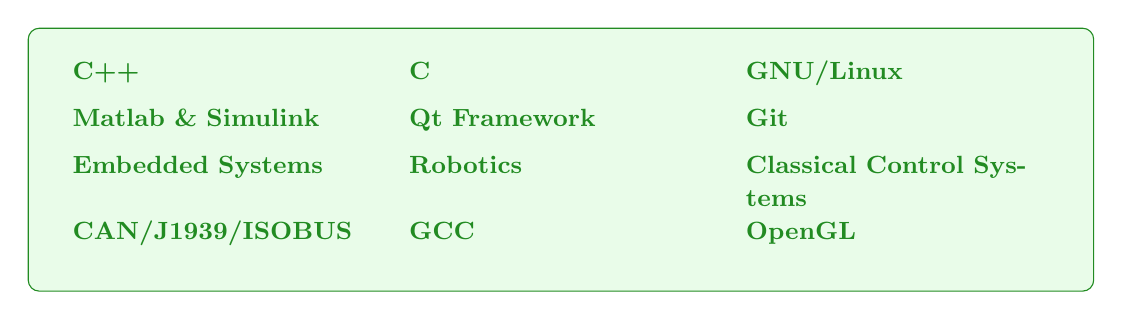
\begin{tikzpicture}
\node[rectangle,draw=forestgreen,rounded corners,inner sep=10pt,fill=lightgreen!20,text width=\textwidth+20pt] {
\begin{tabularx}{\textwidth}{XXX}
\skill{C++} & \skill{C} & \skill{GNU/Linux} \\[5pt]
\skill{Matlab \& Simulink} & \skill{Qt Framework} & \skill{Git} \\[5pt]
\skill{Embedded Systems} & \skill{Robotics} & \skill{Classical Control Systems} \\[5pt]
\skill{CAN/J1939/ISOBUS} & \skill{GCC} & \skill{OpenGL} \\[5pt]
\end{tabularx}
};
\end{tikzpicture}

% Experience Section
\section{Experience}

% Add some vertical space before first company
\vspace{2pt}
\employer{Ag Leader Technology}{Staff Software Engineer}{2018 - Present}
\noproject{Currently implementting agricultureal vehicle automation system using VPI AprilTag Detector on NVIDIA Jetson}
\project{In-Cab Touchscreen Display -- InCommand Go}{-Lead development of next-generation precision agriculture displays, implementing advanced 3D mapping engine using Qt3D and OpenGL in an embedded Linux environment (i.MX8 QM)\\
    -Integrate new 3D map engine with legacy codebase while optimizing for graphics performance using available software profiling tools.
    -Develop custom OpenGL ES shaders for improved rendering performance.
}
\project{Liquid Application Control -- L2 \& RightSpot}{-Create proprietary liquid application control system for precision agriculture sprayer.\\
    -Develop controls for liquid pressure control and flow rate control for servo and pwm valves.\\
    -Design a CAN protocol to communicate with 3rd party pwm nozzle by nozzle sprayer system and develop controls for nozzle duty-cycle.\\
    -Design and implement software for integrating with OEM vehicles over j1939 as well as simulators for testing and implementing the vehicle integration.
}
\project{High Speed Planting -- SureSpeed}{-Create new high-speed planting system using BLDC motors for seed meter and seed tube and proprietary sensors communicating over j1939.\\
    -Implement touch based user interface for in-cab display for improved diagnostic features.
}
\employer{Randstad Technologies}{Software Engineer}{2017 - 2018}
\project{Caterpillar -- Core Machine Software}{Create desktop ecosystem for running embedded code interfacing with Simulink, C\#, C++, and GTest}
\employer{Caterpillar, Inc.}{Software Engineer}{2013 - 2016}
\project{Drivetrain Systems \& Software - Large Mining Trucks}{Powershift transmission clutch control using C and Simulink}


% Education Section
\section{Education}
\employer{Iowa State University}{B.S. Electrical Engineering}{2012}
% Volunteer Section
\section{Volunteer Experience}
\employer{FIRST Robotics Competition}{Mentor}{}
\volunteer{Team Neutrino 4H}{Lead Mentor (Controls)}{2012, 2020 - Present}
\volunteer{Robot Casserole}{Mechanical Mentor}{2013 - 2016}

\end{document}
